%%%%%%%%%%%%%%%%%%%%%%%%%%%%%%%%%%%%%%%%%%%%%%%%%%%%%%%%%%%%%%%%%%%%%%%%%%%%%%%%
%%%%%%%%%%%%%%%%%%%%%%%%%%%%%%%%%%%%%%%%%%%%%%%%%%%%%%%%%%%%%%%%%%%%%%%%%%%%%%%%
%%                                                                            %%
%% thesistemplate.tex version 3.20 (2018/08/31)                               %%
%% The LaTeX template file to be used with the aaltothesis.sty (version 3.20) %%
%% style file.                                                                %%
%% This package requires pdfx.sty v. 1.5.84 (2017/05/18) or newer.            %%
%%                                                                            %%
%% This is licensed under the terms of the MIT license below.                 %%
%%                                                                            %%
%% Written by Luis R.J. Costa.                                                %%
%% Currently developed at the Learning Services of Aalto University School of %%
%% Electrical Engineering by Luis R.J. Costa since May 2017.                  %%
%%                                                                            %%
%% Copyright 2017-2018, by Luis R.J. Costa, luis.costa@aalto.fi,              %%
%% Copyright 2017-2018 Swedish translations in aaltothesis.cls by Elisabeth   %%
%% Nyberg, elisabeth.nyberg@aalto.fi and Henrik Wallén,                       %%
%% henrik.wallen@aalto.fi.                                                    %%
%% Copyright 2017-2018 Finnish documentation in the template opinnatepohja.tex%%
%% by Perttu Puska, perttu.puska@aalto.fi, and Luis R.J. Costa.               %%
%% Copyright 2018 English template thesistemplate.tex by Luis R.J. Costa.     %%
%% Copyright 2018 Swedish template kandidatarbetsbotten.tex by Henrik Wallen. %%
%%                                                                            %%
%% Permission is hereby granted, free of charge, to any person obtaining a    %%
%% copy of this software and associated documentation files (the "Software"), %%
%% to deal in the Software without restriction, including without limitation  %%
%% the rights to use, copy, modify, merge, publish, distribute, sublicense,   %%
%% and/or sell copies of the Software, and to permit persons to whom the      %%
%% Software is furnished to do so, subject to the following conditions:       %%
%% The above copyright notice and this permission notice shall be included in %%
%% all copies or substantial portions of the Software.                        %%
%% THE SOFTWARE IS PROVIDED "AS IS", WITHOUT WARRANTY OF ANY KIND, EXPRESS OR %%
%% IMPLIED, INCLUDING BUT NOT LIMITED TO THE WARRANTIES OF MERCHANTABILITY,   %%
%% FITNESS FOR A PARTICULAR PURPOSE AND NONINFRINGEMENT. IN NO EVENT SHALL    %%
%% THE AUTHORS OR COPYRIGHT HOLDERS BE LIABLE FOR ANY CLAIM, DAMAGES OR OTHER %%
%% LIABILITY, WHETHER IN AN ACTION OF CONTRACT, TORT OR OTHERWISE, ARISING    %%
%% FROM, OUT OF OR IN CONNECTION WITH THE SOFTWARE OR THE USE OR OTHER        %%
%% DEALINGS IN THE SOFTWARE.                                                  %%
%%                                                                            %%
%%                                                                            %%
%%%%%%%%%%%%%%%%%%%%%%%%%%%%%%%%%%%%%%%%%%%%%%%%%%%%%%%%%%%%%%%%%%%%%%%%%%%%%%%%
%%                                                                            %%
%%                                                                            %%
%% An example for writting your thesis using LaTeX                            %%
%% Original version and development work by Luis Costa, changes to the text   %% 
%% in the Finnish template by Perttu Puska.                                   %%
%% Support for Swedish added 15092014                                         %%
%% PDF/A-b support added on 15092017                                          %%
%% PDF/A-2 support added on 24042018                                          %%
%%                                                                            %%
%% This example consists of the files                                         %%
%%         thesistemplate.tex (version 3.20) (for text in English)            %%
%%         opinnaytepohja.tex (version 3.20) (for text in Finnish)            %%
%%         kandidatarbetsbotten.tex (version 1.00) (for text in Swedish)      %%
%%         aaltothesis.cls (versio 3.20)                                      %%
%%         kuva1.eps (graphics file)                                          %%
%%         kuva2.eps (graphics file)                                          %%
%%         kuva1.jpg (graphics file)                                          %%
%%         kuva2.jpg (graphics file)                                          %%
%%         kuva1.png (graphics file)                                          %%
%%         kuva2.png (graphics file)                                          %%
%%         kuva1.pdf (graphics file)                                          %%
%%         kuva2.pdf (graphics file)                                          %%
%%                                                                            %%
%%                                                                            %%
%% Typeset in Linux either with                                               %%
%% pdflatex: (recommended method)                                             %%
%%             $ pdflatex thesistemplate                                      %%
%%             $ pdflatex thesistemplate                                      %%
%%                                                                            %%
%%   The result is the file thesistemplate.pdf that is PDF/A compliant, if    %%
%%   you have chosen the proper \documenclass options (see comments below)    %%
%%   and your included graphics files have no problems.
%%                                                                            %%
%% Or                                                                         %%
%% latex: (this method is not recommended)                                    %%
%%             $ latex thesistemplate                                         %%
%%             $ latex thesistemplate                                         %%
%%                                                                            %%
%%   The result is the file thesistemplate.dvi, which is converted to ps      %%
%%   format as follows:                                                       %%
%%                                                                            %%
%%             $ dvips thesistemplate -o                                      %%
%%                                                                            %%
%%   and then to pdf as follows:                                              %%
%%                                                                            %%
%%             $ ps2pdf thesistemplate.ps                                     %%
%%                                                                            %%
%%   This pdf file is not PDF/A compliant. You must must make it so using,    %%
%%   e.g., Acrobat Pro or PDF-XChange.                                        %%
%%                                                                            %%
%%                                                                            %%
%% Explanatory comments in this example begin with the characters %%, and     %%
%% changes that the user can make with the character %                        %%
%%                                                                            %%
%%%%%%%%%%%%%%%%%%%%%%%%%%%%%%%%%%%%%%%%%%%%%%%%%%%%%%%%%%%%%%%%%%%%%%%%%%%%%%%%
%%%%%%%%%%%%%%%%%%%%%%%%%%%%%%%%%%%%%%%%%%%%%%%%%%%%%%%%%%%%%%%%%%%%%%%%%%%%%%%%
%%
%% WHAT is PDF/A
%%
%% PDF/A is the ISO-standardized version of the pdf. The standard's goal is to
%% ensure that he file is reproducable even after a long time. PDF/A differs
%% from pdf in that it allows only those pdf features that support long-term
%% archiving of a file. For example, PDF/A requires that all used fonts are
%% embedded in the file, whereas a normal pdf can contain only a link to the
%% fonts in the system of the reader of the file. PDF/A also requires, among
%% other things, data on colour definition and the encryption used.
%% Currently three PDF/A standards exist:
%% PDF/A-1: based on PDF 1.4, standard ISO19005-1, published in 2005.
%%          Includes all the requirements essential for long-term archiving.
%% PDF/A-2: based on PDF 1.7, standard ISO19005-2, published in 2011.
%%          In addition to the above, it supports embedding of OpenType fonts,
%%          transparency in the colour definition and digital signatures.
%% PDF/A-3: based on PDF 1.7, standard ISO19005-3, published in 2012.
%%          Differs from the above only in that it allows embedding of files in
%%          any format (e.g., xml, csv, cad, spreadsheet or wordprocessing
%%          formats) into the pdf file.
%% PDF/A-1 files are not necessarily PDF/A-2 -compatible and PDF/A-2 are not
%% necessarily PDF/A-1 -compatible.
%% All of the above PDF/A standards have two levels:
%% b: (basic) requires that the visual appearance of the document is reliably
%%    reproduceable.
%% a (accessible) in addition to the b-level requirements, specifies how
%%   accessible the pdf file is to assistive software, say, for the physically
%%   impaired.
%% For more details on PDF/A, see, e.g., https://en.wikipedia.org/wiki/PDF/A
%%
%%
%% WHICH PDF/A standard should my thesis conform to?
%%
%% Primarily to the PDF/A-1b standard. All the figures and graphs typically
%% use in thesis work do not require transparency features, a basic '2-D'
%% visualisation suffices. The font to be used are specified in this template
%% and they should not be changed. However, if you have figures where
%% transparency characteristics matter, use the PDF/A-2b standard. Do not use
%% the PDF/A-3b standard for your thesis.
%%
%%
%% WHAT graphics format can I use to produce my PDF/A compliant file?
%%
%% When using pdflatex to compile your work, use jpg, png or pdf files. You may
%% have PDF/A compliance problems with figures in pdf format. Do not use PDF/A
%% compliant graphics files.
%% If you decide to use latex to compile your work, the only acceptable file
%% format for your figure is eps. DO NOT use the ps format for your figures.

%% USE one of these:
%% * the first when using pdflatex, which directly typesets your document in the
%%   chosen pdf/a format and you want to publish your thesis online,

%% * the second when you want to print your thesis to bind it, or
%% * the third when producing a ps file and a pdf/a from it.
%%
\documentclass[english, 12pt, a4paper, elec, utf8, a-1b, online]{aaltothesis}
%\documentclass[english, 12pt, a4paper, elec, utf8, a-1b]{aaltothesis}
%\documentclass[english, 12pt, a4paper, elec, dvips, online]{aaltothesis}

%% Use the following options in the \documentclass macro above:
%% your school: arts, biz, chem, elec, eng, sci
%% the character encoding scheme used by your editor: utf8, latin1
%% thesis language: english, finnish, swedish
%% make an archiveable PDF/A-1b or PDF/A-2b compliant file: a-1b, a-2b
%%                    (with pdflatex, a normal pdf containing metadata is
%%                     produced without the a-*b option)
%% typeset in symmetric layout and blue hypertext for online publication: online
%%            (no option is the default, resulting in a wide margin on the
%%             binding side of the page and black hypertext)
%% two-sided printing: twoside (default is one-sided printing)
%%

%% Use one of these if you write in Finnish (see the Finnish template
%% opinnaytepohja.tex)
%\documentclass[finnish, 12pt, a4paper, elec, utf8, a-1b, online]{aaltothesis}
%\documentclass[finnish, 12pt, a4paper, elec, utf8, a-1b]{aaltothesis}
%\documentclass[finnish, 12pt, a4paper, elec, dvips, online]{aaltothesis}

\usepackage{graphicx}

%% Math fonts, symbols, and formatting; these are usually needed
\usepackage{amsfonts,amssymb,amsbsy,amsmath}

%% Change the school field to specify your school if the automatically set name
%% is wrong
% \university{aalto-yliopisto}
% \school{Sähkötekniikan korkeakoulu}

%% Edit to conform to your degree programme
%%
\degreeprogram{Automation and Electrical Engineering}
%%

%% Your major
%%
\major{Control, Robotics and Autonomous Systems}
%%

%% Major subject code
%%
\code{ELEC3025}
%%
 
%% Choose one of the three below
%%
%\univdegree{BSc}
\univdegree{MSc}
%\univdegree{Lic}
%%

%% Your name (self explanatory...)
%%
\thesisauthor{Saidnassimov Darkhan}
%%

%% Your thesis title comes here and possibly again together with the Finnish or
%% Swedish abstract. Do not hyphenate the title, and avoid writing too long a
%% title. Should LaTeX typeset a long title unsatisfactorily, you mght have to
%% force a linebreak using the \\ control characters.
%% In this case...
%% Remember, the title should not be hyphenated!
%% A possible "and" in the title should not be the last word in the line, it
%% begins the next line.
%% Specify the title again without the linebreak characters in the optional
%% argument in box brackets. This is done because the title is part of the 
%% metadata in the pdf/a file, and the metadata cannot contain linebreaks.
%%
\thesistitle{Equipment identification through image recognition}
%\thesistitle[Title of the thesis]{Title of\\ the thesis}
%%

%%
\place{Espoo}
%%

%% The date for the bachelor's thesis is the day it is presented
%%
\date{10.7.2022}
%%

%% Thesis supervisor
%% Note the "\" character in the title after the period and before the space
%% and the following character string.
%% This is because the period is not the end of a sentence after which a
%% slightly longer space follows, but what is desired is a regular interword
%% space.
%%
\supervisor{Prof.\ Alexander Ilin}
%%

%% Advisor(s)---two at the most---of the thesis. Check with your supervisor how
%% many official advisors you can have.
%%
\advisor{Dr Christian Binder}
%\advisor{MSc Sarah Scientist}
%%

%% Aaltologo: syntax:
%% \uselogo{aaltoRed|aaltoBlue|aaltoYellow|aaltoGray|aaltoGrayScale}{?|!|''}
%% The logo language is set to be the same as the thesis language.
%%
\uselogo{aaltoRed}{''}
%%

%% The English abstract:
%% All the details (name, title, etc.) on the abstract page appear as specified
%% above.
%% Thesis keywords:
%% Note! The keywords are separated using the \spc macro
%%
\keywords{Computer vision\spc domain adaptation\spc object detection\spc 3D models}
%%

%% The abstract text. This text is included in the metadata of the pdf file as well
%% as the abstract page.
%%
\thesisabstract{
Your abstract in English. Keep the abstract short. The abstract explains your 
research topic, the methods you have used, and the results you obtained. In the 
PDF/A format of this thesis, in addition to the abstract page, the abstract text is 
written into the pdf file's metadata. Write here the text that goes into the 
metadata. The metadata cannot contain special characters, linebreak or paragraph 
break characters, so these must not be used here. If your abstract does not contain 
special characters and it does not require paragraphs, you may take advantage of 
the abstracttext macro (see the comment below). Otherwise, the metadata abstract 
text must be identical to the text on the abstract page.
}

%% Copyright text. Copyright of a work is with the creator/author of the work
%% regardless of whether the copyright mark is explicitly in the work or not.
%% You may, if you wish, publish your work under a Creative Commons license (see
%% creaticecommons.org), in which case the license text must be visible in the
%% work. Write here the copyright text you want. It is written into the metadata
%% of the pdf file as well.
%% Syntax:
%% \copyrigthtext{metadata text}{text visible on the page}
%% 
%% In the macro below, the text written in the metadata must have a \noexpand
%% macro before the \copyright special character, and macros (\copyright and
%% \year here) must be separated by the \ character (space chacter) from the
%% text that follows. The macros in the argument of the \copyrighttext macro
%% automatically insert the year and the author's name. (Note! \ThesisAuthor is
%% an internal macro of the aaltothesis.cls class file).
%% Of course, the same text could have simply been written as
%% \copyrighttext{Copyright \noexpand\copyright\ 2018 Eddie Engineer}
%% {Copyright \copyright{} 2018 Eddie Engineer}
%%
\copyrighttext{Copyright \noexpand\copyright\ \number\year\ \ThesisAuthor}
{Copyright \copyright{} \number\year{} \ThesisAuthor}

%% You can prevent LaTeX from writing into the xmpdata file (it contains all the 
%% metadata to be written into the pdf file) by setting the writexmpdata switch
%% to 'false'. This allows you to write the metadata in the correct format
%% directly into the file thesistemplate.xmpdata.
%\setboolean{writexmpdatafile}{false}

%% All that is printed on paper starts here
%%
\begin{document}

%% Create the coverpage
%%
\makecoverpage

%% Typeset the copyright text.
%% If you wish, you may leave out the copyright text from the human-readable
%% page of the pdf file. This may seem like a attractive idea for the printed
%% document especially if "Copyright (c) yyyy Eddie Engineer" is the only text
%% on the page. However, the recommendation is to print this copyright text.
%%
\makecopyrightpage

%% Note that when writting your thesis in English, place the English abstract
%% first followed by the possible Finnish or Swedish abstract.

%% Abstract text
%% All the details (name, title, etc.) on the abstract page appear as specified
%% above.
%%
%%\begin{abstractpage}[english]
%%  Your abstract in English. Keep the abstract short. The abstract explains your
%%  research topic, the methods you have used, and the results you obtained.  
  
%%  The abstract text of this thesis is written on the readable abstract page as
%%  well as into the pdf file's metadata via the $\backslash$thesisabstract macro
%%  (see above). Write here the text that goes onto the readable abstract page.
%%  You can have special characters, linebreaks, and paragraphs here. Otherwise,
%%  this abstract text must be identical to the metadata abstract text.
  
%%  If your abstract does not contain special characters and it does not require
%%  paragraphs, you may take advantage of the abstracttext macro (see the comment
%%  below).
%%\end{abstractpage}

%% The text in the \thesisabstract macro is stored in the macro \abstractext, so
%% you can use the text metadata abstract directly as follows:
%%
\begin{abstractpage}[english]
	\abstracttext{}
\end{abstractpage}


%% Preface
%%
%% This section is optional. Remove it if you do not want a preface.
\mysection{Preface}
%\mysection{Esipuhe}
I would like to thank Professor Alexander Ilin at Aalto University for his excellent guidance. Additionally, I would like to thank Dr Christian Binder for offering the opportunity at Metso Outotec and providing full support throughout the process. Finally, I would like to thank the CSC Finnish IT center for science for the computing resources that made the research possible. \\

\vspace{5cm}
Otaniemi, 10.7.2022

\vspace{5mm}
{\hfill Saidnassimov, D.\hspace{1cm}}

%% Force a new page after the preface
%%
\newpage


%% Table of contents. 
%%
\thesistableofcontents

\cleardoublepage
\subsection*{List of Figures}
\cleardoublepage
\subsection*{List of Tables}
\cleardoublepage

%% Symbols and abbreviations
\mysection{Symbols and abbreviations}

\subsection*{Symbols}

\begin{tabular}{ll}
$\mathbf{B}$  & magnetic flux density  \\
$c$              & speed of light in vacuum $\approx 3\times10^8$ [m/s]\\
$\omega_{\mathrm{D}}$    & Debye frequency \\
$\omega_{\mathrm{latt}}$ & average phonon frequency of lattice \\
$\uparrow$       & electron spin direction up\\
$\downarrow$     & electron spin direction down
\end{tabular}

\subsection*{Operators}

\begin{tabular}{ll}
$\nabla \times \mathbf{A}$              & curl of vectorin $\mathbf{A}$\\
$\displaystyle\frac{\mbox{d}}{\mbox{d} t}$ & derivative with respect to 
variable $t$\\[3mm]
$\displaystyle\frac{\partial}{\partial t}$  & partial derivative with respect 
to variable $t$ \\[3mm]
$\sum_i $                       & sum over index $i$\\
$\mathbf{A} \cdot \mathbf{B}$    & dot product of vectors $\mathbf{A}$ and 
$\mathbf{B}$
\end{tabular}

\subsection*{List of Abbreviations}


\begin{tabular}{ll}
AC         & alternating current \\
APLAC      & an object-oriented analog circuit simulator and design tool \\
           & (originally Analysis Program for Linear Active Circuits) \\
BCS        & Bardeen-Cooper-Schrieffer \\ %% dash between the names
DC         & direct current \\
TEM        & transverse eletromagnetic
\end{tabular}


%% \clearpage is similar to \newpage, but it also flushes the floats (figures
%% and tables).
%%
\cleardoublepage

%% Text body begins. Note that since the text body is mostly in Finnish the
%% majority of comments are also in Finnish after this point. There is no point
%% in explaining Finnish-language specific thesis conventions in English.
%% This text will be translated to English soon.
%%
\section{Introduction}

%% Leave page number of the first page empty
%% 
\thispagestyle{empty}
\subsection*{Problem statement}
In recent years, computer vision algorithms have received much attention due to their potential applications in a vast variety of fields. As the technologies advance, endless possiblities arise in numerous fields, such as security monitoring, medicine and self driving vehicles. \cite{Oza2021} Although over the last decade computer vision has been emerging in indurstial applications, such as safety and process monitoring \cite{Oza2021}, fewer research has addressed the issue of equipment detection. 

Industrial plants typically are hundreds of meters long and often it becomes frustrating to identify minor equipment parts. Identifying the parts becomes relevant once they need replacement or maintenance as the plant would not be able to run at full capacity without them. Ore processing plants treat several hundreds of tons of ore per hour, and the production capacity is constant. \cite{Oza2021}. Therefore, quite often it is troublesome to properly identify the equipment within a list of thousands of various parts in a medium to large scaled plant. 

Although various methods have been implemented for detection of objects in various domains\cite{Oza2021}, these methods require an extensive dataset of images in order to work. In our scenario, the images can easily be collected from the simulator, however, this raises certain restrictions on the accuracy of the models as the models will not perform as well on real images.  

This thesis proposes feasible object detection algorithms as a solution to automatically localize and identify the equipment in a large environment and minimize the delay before the production is online again. 

\subsection*{Thesis objective}
The aim of the thesis is to identify a suitable object detection method for an industrial environment and develop a minimal proof of concept application with user interface. The selected method should be able to identify an object in a real image given a dataset of rendered images from a 3D equipment model.

Additionally, a method should propose a solution to optimize the laborous data collection and labelling process. The optimization is important not only because it is a time demanding process, but also because in large plants there are thousands of objects and scalability is critical. 

\subsection*{Methods}

In order to accomplish the objectives defined, this paper will compare multiple methods for object detection and explore the most recent developments in domain adaptation field. 
For the purpose of training an object detection model, a vast number of training and testing pictures is required. In most traditional object detection algorithms, there is little to no difference in the environment where the training and testing images have been taken. Unfortunately, often the accuracy results  are lower than anticipated, when the phenomenon of domain shift takes place. \cite{Oza2021} Domain shift occurs, for example, when the object of interest is placed under different weather or lighting conditions, such as \cite{Oza2021}.
Additionally, in an industrial environment, it often becomes challenging to take pictures due to accessibility and confidentiality regulations. Therefore, this paper proposes to tackle the challenge by means of domain adaptation, namely Cross Domain Adaptation,  Decoupled Adaptation for Cross Domain Object Detection and Progressive Domain Adaptation for Object Detection. 
The dataset utilized to implement the methods is based on TLess open source dataset\cite{Oza2021} due to limitations in obtaining real life data. Originally the dataset is meant for pose estimation in 3D models, therefore the dataset was converted to formats, appropriate for the proposed methods. 

The methods will be trained on rendered data from 3D models and evaluated on real images using mean average precision metrics. 
Finally, the selected method will be evaluated on one equipment item from a real plant. 

\subsection*{Scope}

The thesis is limited to proposing the solution upon analysing multiple existing state-of-the-art methodologies. Preparing the actual real life dataset and implementing the solution for a real plant remains out of the scope. Although the proposed methods attempt to minimize the data collection and labelling process, it might take multiple months before a model based on the real data is ready for training. 
 
\subsection*{Metso:Outotec}
The issuer and the commissioner of the thesis topic is Metso Outotec Oyj. Metso Outotec is a Finnish publicly traded company that formed as a result of a merger of two companies - Metso Minerals and Outotec on June, 2020. The company provides sustainable solutions and services worldwide for minerals processing, aggregates and metal refining. 

Along with the focus on sustainability and strive for innovation, Metso Outotec aims on digitization throughout the equipment cycle. Therefore, the company offers various IoT solutions that attempt to optimize various production processes for customers. \cite{Oza2021} Naturally, computer vision is of great interest to the company due to its potential in the industry and the proposed thesis topic was reported to be in high demand among the plant owners.

%https://www.mogroup.com/corporate/
%https://www.mogroup.com/corporate/about-us/

\subsection*{Structure of the thesis}

The rest of this thesis is divided into five chapters. Chapter 2 reviews the literature relevant to understand the main concepts and algorithms used during the research. Chapter 3 outlines the methodology and the analysis of the proposed computer vision solutions. Chapter 4 evaluates the solution and presents the results of the thesis using different metrics. Chapter 5 summarizes the works by discussing the accuracy of the proposed models as well as suggesting directions for future work.  

% or \begin{enumerate}
%\begin{itemize}
%\item[--]Relevance
%\item[--]Current practices
%\item[--]Existing solutions
%\item[--]Problems
%\item[--]Aim
%\item[--]Methods
%\item[--]Scope
%\item[--]Structure
%\end{itemize}

%%T\"am\"an 

%% In a thesis, every section starts a new page, hence \clearpage
\clearpage
\section{Related work}
TODO
\subsection*{Computer vision}
TODO
\subsection*{Deep convolutional neural networks}
TODO
\subsection*{Object detection}
TODO
\subsection*{Domain adaptation}
TODO
\subsection*{Domain Adaptive Object Detection}
TODO
%% Three levels of hierarchy in sectioning should be enough
\subsection*{Adversarial feature learning}
TODO
\subsection*{Pseudo-label based self-training}
TODO
\subsection*{Image-to-image translation}
TODO
\subsection*{Domain randomization}
TODO
\subsection*{Mean teacher training}
TODO
\subsection*{Graph-reasoning}
TODO


\section{Research Methodology}
%\section{Tutkimusaineisto ja -menetelm\"at}

TODO
\subsection*{Proposed method}
TODO

\subsection*{Implementation details}
TODO

\subsection*{Dataset}
TODO \cite{Li2020}


\section{Validation and Results}
%\section{Tulokset}
TODO

\clearpage

\section{Analysis and Discussion} 

TODO
\clearpage

\section{Conclusion and Future Work} 
%\section{Yhteenveto}

TODO


\clearpage
%% L\"ahdeluettelo



\bibliographystyle{plain}
\bibliography{references_library}

%% Appendices
%% If you don't have appendices, remove \clearpage and \thesisappendix below.
\clearpage

\thesisappendix

\section{Appendices\label{LiiteA}}

Liitteet eiv\"at ole opinn\"aytteen kannalta v\"altt\"am\"att\"omi\"a ja 
opinn\"aytteen tekij\"an on 
kirjoittamaan ryhtyess\"a\"an hyv\"a ajatella p\"arj\"a\"av\"ans\"a ilman liitteit\"a.
Kokemattomat kirjoittajat, jotka ovat huolissaan
tekstiosan pituudesta, paisuttavat turhan 
helposti liitteit\"a pit\"a\"akseen tekstiosan pituuden annetuissa rajoissa.
T\"all\"a tavalla ei synny hyv\"a\"a opinn\"aytett\"a.   

Liite on itsen\"ainen kokonaisuus, vaikka se t\"aydent\"a\"akin tekstiosaa.
Liite ei siten ole pelkk\"a listaus, kuva tai taulukko, vaan 
liitteess\"a selitet\"a\"an aina sis\"all\"on laatu ja tarkoitus. 

Liitteeseen voi laittaa esimerkiksi listauksia. Alla on 
listausesimerkki t\"am\"an liitteen luomisesta. 

%% Verbatim-ymp\"arist\"o ei muotoile tai tavuta teksti\"a. Fontti on monospace.
%% Verbatim-ymp\"arist\"on sis\"all\"a annettuja komentoja ei LaTeX k\"asittele. 
%% Vasta \end{verbatim}-komennon j\"alkeen jatketaan k\"asittely\"a.
\begin{verbatim}
	\clearpage
	\appendix
	\addcontentsline{toc}{section}{Liite A}
	\section*{Liite A}
	...
	\thispagestyle{empty}
	...
	teksti\"a
	...
	\clearpage
\end{verbatim}

Kaavojen numerointi muodostaa liitteiss\"a oman kokonaisuutensa:
\begin{align}
d \wedge A &= F, \label{liitekaava1}\\
d \wedge F &= 0. \label{liitekaava2}
\end{align}


\clearpage
\section{Appendices2\label{LiiteB}}

%% Liitteiden kaavat, taulukot ja kuvat numeroidaan omana kokonaisuutenaan
%%
%% Equations, tables and figures have their own numbering in Appendices
%\renewcommand{\theequation}{B\arabic{equation}}
%\setcounter{equation}{0}  
%\renewcommand{\thefigure}{B\arabic{figure}}
%\setcounter{figure}{0}
%\renewcommand{\thetable}{B\arabic{table}}
%\setcounter{table}{0}

Liitteiss\"a voi my\"os olla kuvia, jotka
eiv\"at sovi leip\"atekstin joukkoon:
%% Ymp\"arist\"on figure parametrit htb pakottavat
%% kuvan t\"ah\"an, eik\"a LaTeX yrit\"a siirrell\"a niit\"a
%% hyv\"aksi katsomaansa paikkaan. 
%% Ymp\"arist\"o\"a center voi k\"aytt\"a\"a \centering-
%% komennon sijaan
%%
%% Example of a figure, note the use of htb parameters which force
%% the figure to be inserted here
\begin{figure}[htb]
\begin{center}
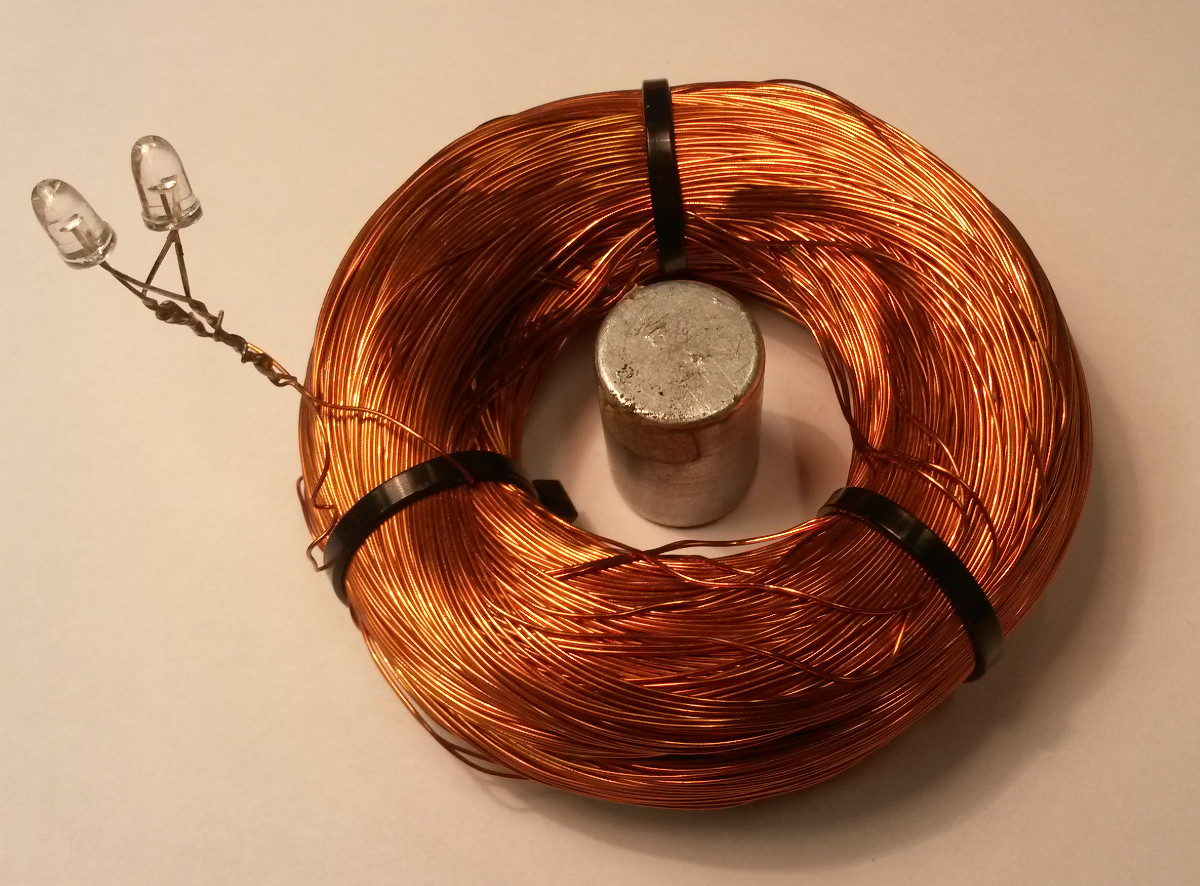
\includegraphics[height=8cm]{./ledspole.jpg}
\end{center}
\caption{Kuvateksti, jossa on liitteen numerointi}
\label{liitekuva}
\end{figure}
%%
Liitteiden taulukoiden numerointi on kuvien ja kaavojen kaltainen:
\begin{table}[htb]
\caption{Taulukon kuvateksti.}
\label{liitetaulukko}
\begin{center}
\fbox{
\begin{tabular}{lp{0.5\linewidth}}
9.00--9.55  & K\"aytett\"avyystestauksen tiedotustilaisuus (osanottajat
ovat saaneet s\"ahk\"opostitse valmistautumisteht\"av\"at, joten tiedotustilaisuus
voidaan pit\"a\"a lyhyen\"a).\\
9.55--10.00 & Testausalueelle siirtyminen
\end{tabular}}
\end{center}
\end{table}
Kaavojen numerointi muodostaa liitteiss\"a oman kokonaisuutensa:
\begin{align}
T_{ik} &= -p g_{ik} + w u_i u_k + \tau_{ik},  \label{liitekaava3} \\
n_i    &= n u_i + v_i.                      \label{liitekaava4}
\end{align}

\section{Temp}
\subsection*{Latex Examples 1}

%% to reference something
%% \label{a} 
%% \ref{a}-\ref{o}

\subsection*{Latex Examples 2}

%% Esimerkki taulukosta
\begin{table}[htb]
%% Taulukon teksti
\caption{Table example \label{taulukko1}}
\begin{center}
\fbox{
\begin{tabular}{c|l|r}
\textbf{A} & 1 & $e^{j \omega t}$ \\ \hline
\textsf{B} & 2 & ${\mathfrak R}(c)$ \\ \hline
\texttt{C} & 3 & $ a \in \mathbb{A}$  
\end{tabular}
}
\end{center}
\end{table}


\subsection*{Latex Examples 3}

\begin{equation}
D(xy) = (Dx)y + x(Dy),  \hspace{3em} x,y \in \mathbb{A}.
\end{equation}
%% The example for embedding the graphics file linediagram.pdf into the document.
%% Command \inclugraphics[parametres]{argument} embeds the graphic.
%% Command \centering centres the graphic on the page horizontally. 
%% Command \caption numbers and places the caption at the position of occurrence.
%% Parameters htb force the figure to the current place of occurrence in the
%% source file, if there is sufficient space, or places it to the top or bottom
%% of the page. 
\begin{figure}[htb]
\centering
%% NOTE! The PDF/A-1b file created when using the jpg, pdf or png file below is
%% error-free. However, with kuva1.pdf, the resulting PDF/A-2b file fails the
%% compliance test in Acrobat Pro but passes it in PDF-XChanger and the validator
%% at https://www.pdf-online.com/osa/validate.aspx tarkistuksen.
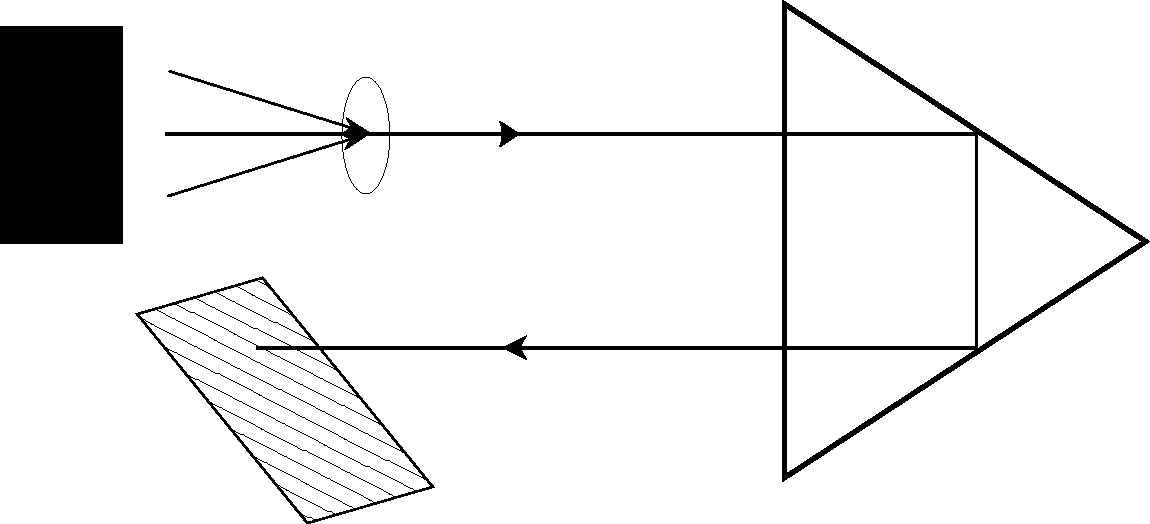
\includegraphics[height=5cm]{./linediagram.pdf}
%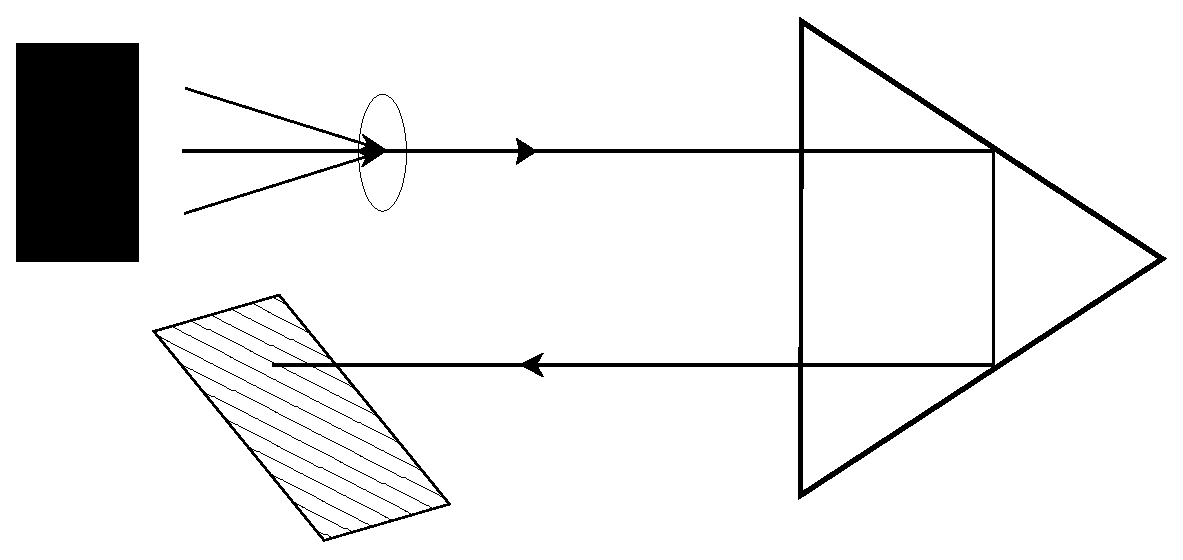
\includegraphics[height=5cm]{./linediagram.eps}
\caption{This is an example of a numbered caption. \label{kuva1}}
\end{figure}

\begin{figure}[htb]
\centering
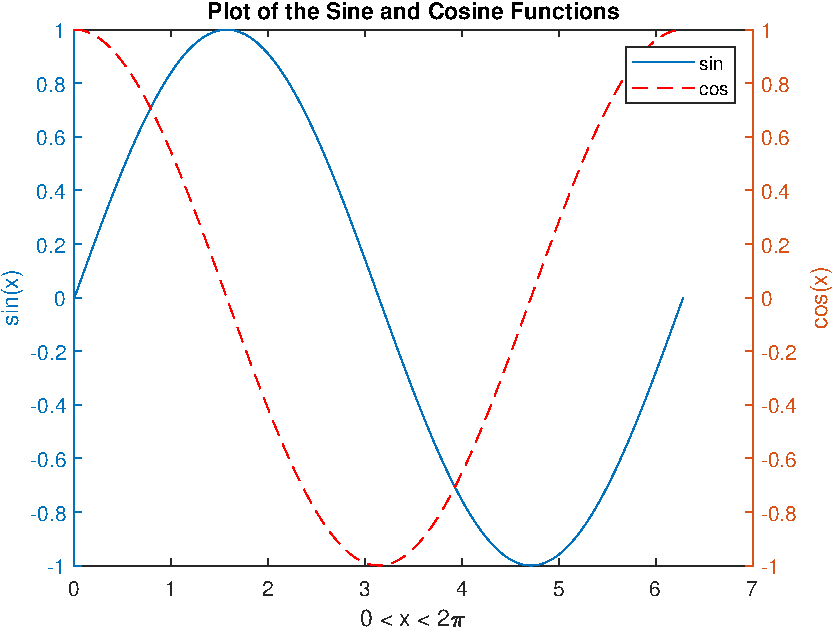
\includegraphics[height=5cm]{curves.pdf}
%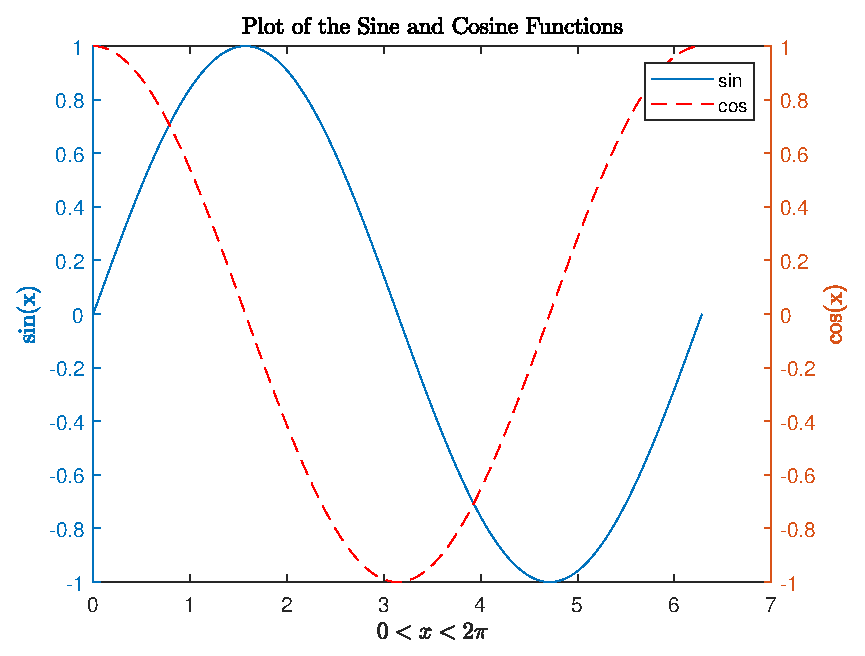
\includegraphics[height=5cm]{curves.eps}
\caption{This is an example of a MATLAB graph. \label{kuva2}}
\end{figure}


\subsection*{Latex Examples 4} 

Footnote example
\footnote{My footnote \underline{ei} } my footnote



\subsection*{Latex Examples 5} 

\textit{italic} blabla

\cite{Oza2021}--\cite{Oza2021}  \cite[s.\ 83--124]{Oza2021}
 

\clearpage
\end{document}
